\chapter{Design and Implementation}

The object-oriented architecture of ToPS was essential for the seamless integration of the models in a single system that included facilities for training, simulating, decoding, integration in GHMMs and construction of Bayesian classifiers.

ToPS's architecture includes  three main class hierarchies:
\textit{ProbabilisticModel}, to represent model implementations; \textit{Probabili\-stic\-ModelCreator}, to specify the on-the fly creation of models based on configuration files;  and \textit{ProbabilisticModelParameterValue}, to enable the parsing of the configuration files. These three hierarchies are used by a set of 13 application programs that implement the framework's user functionalities (\textit{align, bayes\_classifier, choose\_path, evaluate, kullback\_positional, mea \_decoding, posterior\_decoding, posterior\_probabilities, pred\_align, simulate, simulate\_alignment, train, viterbi\_decoding}) .


\section{ProbabilisticModel  hierarchy}

In ToPS every model is implemented as part of ProbabilisticModel hierarchy, shown in Figure~\ref{fig:models}.  At the root of the hierarchy  we have the  abstract class {\it ProbabilisticModel}, with methods that characterize any generative model. In particular, {\it ProbabilisticModel} has two important abstract methods: {\it evaluate}, and {\it choose}. The {\it evaluate} method, in subclasses,  should calculate the probability of a sequence given the model and the {\it choose} method should sample a new sequence given the model. This class is used by other parts of the system to ensure that new probabilistic models are included seamlessly in the framework and benefit from all current functionality.


\begin{figure}[htpb]
  \centering
  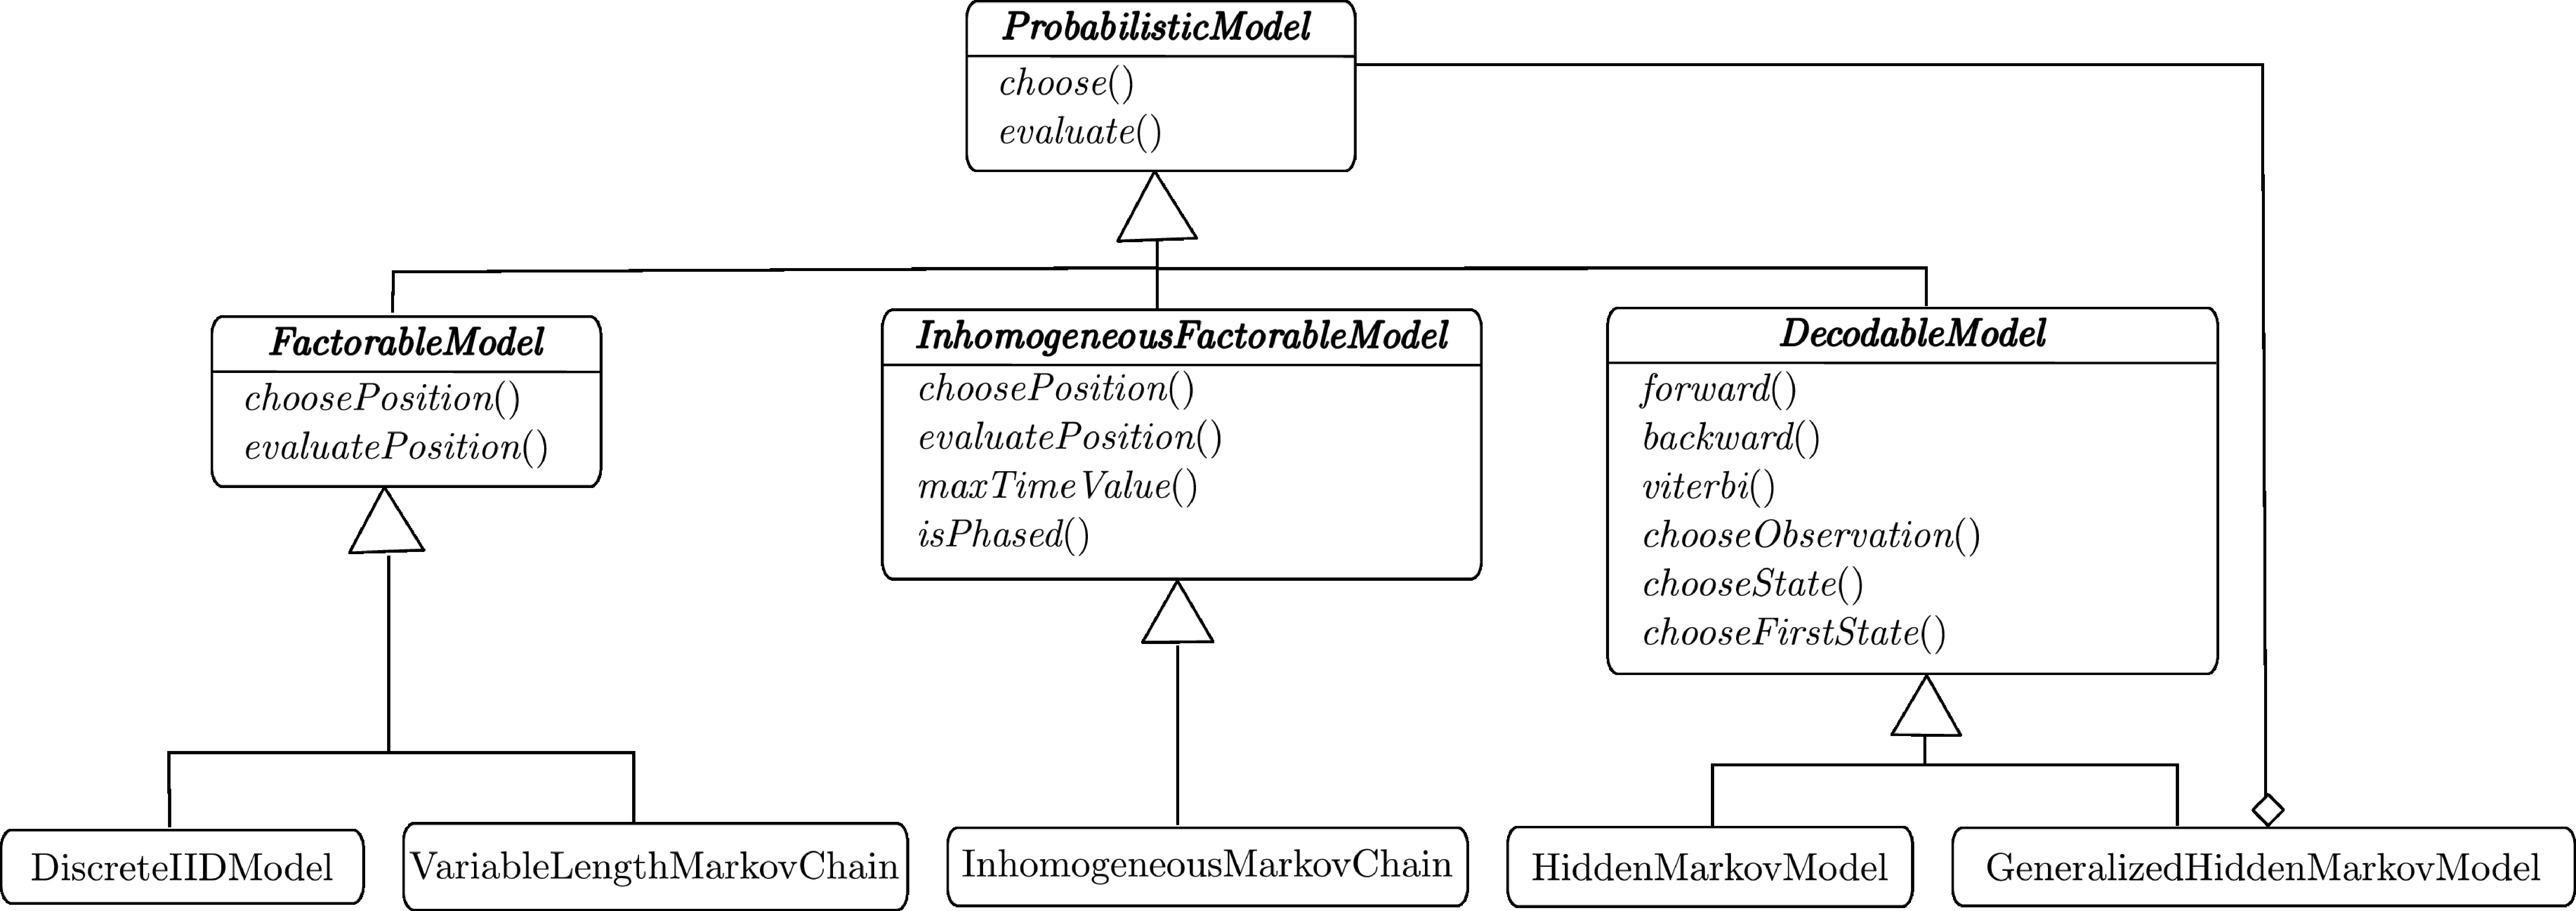
\includegraphics[width=\textwidth]{diagrama_classe}
  \caption{ {\bf Class diagram representing the \textit{ProbabilisticModel} hierarchy.} }
  \label{fig:models}
\end{figure}


%A challenge in the ToPS design was to allow the use  of each model in distinct situations. For example, a HMM can be used in a Bayesian Classifier or as a submodel in a GHMM. This is accomplished with the  classes shown in Figure~\ref{fig:models}.


At the second level of the hierarchy, there are three other abstract classes that implement both the \textit{choose} method, and the \textit{evaluate} method: \textit{FactorableModel}, \textit{Inhomogeneous\-Factorable\-Model}, and \textit{DecodableModel}.

The last level of the hierarchy contains the implementation of the models currently available in ToPS in the form of concrete classes: \textit{DiscreteIIDModel}, \textit{Varia\-bleLengthMarkovChain}, \textit{InhomogeneousMarkovChain},  \textit{Hidden\-Markov\-Model}, \textit{PairHiddenMarkovModel} and  \textit{GeneralizedHidden\-Markov\-Model}.  In particular, \textit{Generalized\-Hidden\-Markov\-Model} uses the {\it Composite}  pattern \cite{Gamma1994}, which guarantees that any new probabilistic model incorporated into the hierarchy  can be  used as a submodel of GHMMs. The implementation of new models will involve extending this hierarchy, and implementing the abstract methods. Using this hierarchy guarantees that new models will work smoothly with the other components of the framework.

In the next  sections we will describe each of the main remaining classes of the hierarchy.



\subsection{FactorableModel}
\label{sec:factorable}

% The knowledge of which models are factorable is important for implementing efficient calculation of emission probabilities as we will se below.

In \textit{FactorableModel}, the \textit{evaluate} method calculates the following formula:

\[ Prob (S|FactorableModel) = \prod_{i=1}^L f(S, i) \]

In which $f$ is a function  of a sequence $S$ and a position $i$ of that sequence. The \textit{choose} method will generate a new sequence by sampling each symbol using the distribution given by the function $f$.

\textit{FactorableModel} also includes two abstract methods: \textit{choose\-Position} and \textit{evaluatePosition}. The \textit{choosePosition} receives a sequence and a position $i$ and samples a new symbol for the position $i$ of the sequence using the function $f$. The \textit{evaluatePosition} receives a sequence and a position $i$ and it returns the probability of the symbol at position $i$ of the sequence using the function $f$. Examples of ``factorable models'' are:

 \begin{itemize}
\item \textit{VariableLengthMarkovChain}, which can capture variable-length dependencies. The function $f$ in this case is equal to:

\[ f_{VLMC}(s, i) = p(s_i|s_{i-1}\cdots s_{i-l})  \]

Where $p(s_i|s_{i-1}\cdots s_{i-l})$ is the probability of the symbol $s_i$ given the past sequence, and $l = l(s_{i-1}, \cdots, s_1)$ is itself a function for the past.

 \item \textit{DiscreteIIDModel}, which is equivalent to order zero Markov chains, where $l = 0$. The function $f$ for this model is:

\[ f_{DiscreteIID}(s,i) = p(s_i) \]

Where $0 \leq p(\sigma) \leq 1$ is the probability of the letter $\sigma \in \Sigma$.

\end{itemize}

Although  \textit{DiscreteIIDModel} is equivalent to the zero order Markov chain, we have chosen to independently implement it, because it provides more efficient algorithms for sampling symbols when $l=0$. We have also implemented training procedure that generates other types of Markov models:

\begin{itemize}
\item Fixed Length Markov Chains of order $k$ can be implemented as a \textit{VariableLengthMarkovChain} where $l=k$ for all the past sequences.

\item Interpolated Markov Model of order $k$ is a Fixed Length Markov Models of order $k$, in which the probability of observing $s_i$ for  context patterns $s_{i-k} \cdots s_{i-1}$ was estimated by interpolating the estimates of smaller context patterns $s_{i-j-k} \cdots s_{i-1}$ ($0\leq j \leq k+1$)~\cite{Salzberg1998}.

\end{itemize}



\subsection{InhomogeneousFactorableModel}
\label{sec:inhomogeneous}

This abstract class rep\-re\-sents models that are time-inhomogeneous, and factorable. In this class the \textit{evaluate} method calculates the following formula:

\begin{align}
Prob(S|InhomogeneousFactorableModel)  =  \prod_{i=1}^L g_t(S, i)
\end{align}

where $g$ is a function of the sequence $S$, a position $i \in \{1,\cdots,L\}$, and a time $t \in \{0, \cdots,  M-1\}$ ($M-1$ is the maximum value of $t$). The \textit{choose} method will sample a new sequence by sampling each symbol for a specific time using the distribution given by the function $g$. Times can be used, for example, to determine different distributions for each codon position in a DNA sequence. 

%The other abstract methods are:
%\begin{itemize}
%\item \textit{choosePosition}, that receives a sequence, a position $i$ and a time $t$,  it chooses a new symbol for the position $i$ of the sequence using the distribution for the time $t$. 
%\item \textit{evaluatePosition}, that receives a sequence, a position $i$ and a time $t$, it returns the probability of the symbol at position $i$ of the sequence using the distribution for the time $t$. 
%\item \textit{isPhased}, that returns a boolean value, when it is true the model represents sequences with arbitrary length by cycling using the distribution of times $0,\cdots,maxTimeValue$.
%\end{itemize}

ToPS currently implement only one subclass of the InhomogeneousFactorableModel, \textit{InhomogeneousMarkovChain} for which the $g$ function is:

\[ g_t(s, i) = p_t (s_i| s_{i-1}\cdots s_{i-l}) \]

here $p_t(s_i|s_{i-1}\cdots s_{i-l})$ is the probability of the symbol $s_i$ for the time $t$ and given the past sequence. The time $t = t(i)$ is itself a function for the position, $t(i) = (i-1) \mod   M$, and order $l = l(s_{i-1} \cdots s_1)$ is itself a function for the past.

Inhomogeneous Markov chains are widely used in Bioinformatics, of which the most notable examples are:
\begin{itemize}
\item {\bf Weight Matrix Model} \cite{Staden1984}, which is an \textit{Inhomogeneou\-Markov\-Chain} of order zero, $l = 0$ for all the past sequences.
\item {\bf Weight Array Model} \cite{Zhang1993}, which  is an \textit{Inhomogeneous\-Markov\-Chain} with order greater than zero, $l = k$ for all the past sequences, $k$ is a constant greater than zero.
\item {\bf Three-periodic Markov Chain} \cite{Borodovsky1993}, which  is an \textit{Inhomogeneous\-Markov\-Chain} with $M$ equals to three and isPhased is true.
\end{itemize}

ToPS provides specific training algorithms to create any of these models as an \textit{InhomogeneousMarkovChain}.

\subsection{DecodableModel}
\label{sec:decodable}

This abstract class represents  models that are used to decode sequences. Hidden Markov Model and Generalized Hidden Markov Model are examples of decodable models. There are three important algorithm for these models:

\begin{itemize}
\item \textbf{forward} algorithm, that calculates the probability $\alpha_k(i)$ of observing the sequence $s_1\cdots s_i$ and ending in state $k$ at position $i$.
\item  \textbf{backward} algorithm, that calculates the probability $\beta_k(i)$ of observing the sequence $s_{i+1}\cdots s_L$ given the state $k$ at position $i$.
\item  \textbf{viterbi} algorithm, that calculates the probability $\gamma_k(i)$ of the most probable path ending in state $k$ with observation $s_1\cdots s_i$.
\end{itemize}

In this class, the methods \textit{forward}, \textit{backward}, \textit{viterbi}, \textit{chooseObserva\-tion}, \textit{choose\-State}, and \textit{choose\-First\-State} are abstract methods.

The \textit{evaluate} method is implemented by using the result of the \textit{forward} algorithm, returning the value:
\begin{align}
Prob(S|DecodableModel) = \sum_{k} \alpha_k(L) f(k)
\end{align}
 where $f(k)$ is the probability of terminating in state $k$.

% {\it DecodableModel} implements the \textit{choose} method by using three abstract methods:  \textit{choose\-Observation}, that receives a sequence $s$, a position $i$, and a state $s$, it samples a new string for the position $i$ of the sequence $s$;  \textit{chooseState}, that receives a state and samples the next state; \textit{choose\-First\-State}, that samples the initial state.

ToPS implements two  \textit{Decodable\-Models}: Hidden Markov Model and Generalized Hidden Markov Model.


\section{ProbabilisticModelCreator   and ProbabilisticModelParameterValue   hierarchies }

The \textit{ProbabilisticModelCreator}  abstracts the process of instantiating members of \textit{ProbabilisticModel} hierarchy from configuration files, implementing the {\it Factory Method}  design pattern \cite{Gamma1994}. Training algorithms are concrete classes of this hierarchy.
The \textit{ProbabilisticModelParameterValue} was designed to facilitate the parsing of configuration files and allow them to be close to the mathematical notation of the models. This hierarchy includes 8 concrete classes that can be examined in the system's webpage. 

Additionally,  ToPS uses two classes \textit{Symbol}, and  \textit{Alphabet} that enable the use of any arbitrary discrete input values by the models. Therefore the user can design system that can use as input, nucleotides, aminoacids, codon names, etc. 



